\section{Method} \label{sec:method} 

In this section we will describe the method we have used to solve the Authorship
Verification problem presented. In general there are two methods of representing
each author. There is the instance based approach and the profile based
approach. In the instance based approach each author is represented by a set of
texts they have written while in the profile based approach they are represented
by the sum of the set of texts they have written. The instance based approach is
illustrated in Figure \ref{fig:instance_based} and the profile based approach is
illustrated in Figure \ref{fig:profile_based}.

\begin{figure}[htb]
    \centering
    \textbf{Instance Based Authorship Verification or Authorship Attribution}
    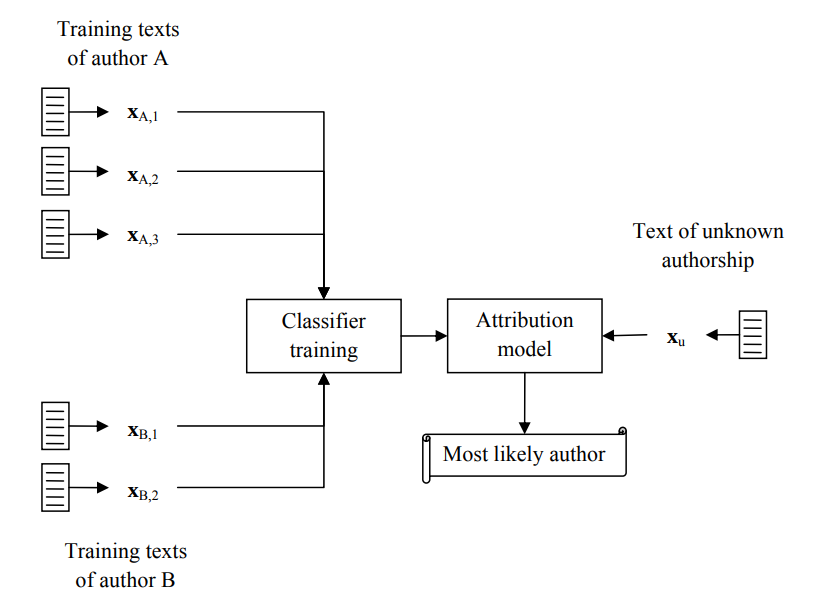
\includegraphics[scale=0.4]{./pictures/method/instance_based.png}

    \caption{Illustrate the typical instance based Authorship Verification or
        Authorship Attribution solution setup.\cite{stamatos2009} A set of
        authors are given as input each with a set of texts. Some Machine
        Learning model is trained on the input texts and the model is used to
        predict an unknown text. }

    \label{fig:instance_based}
\end{figure}

\begin{figure}[htb]
    \centering
    \textbf{Profile Based Authorship Verification or Authorship Attribution}
    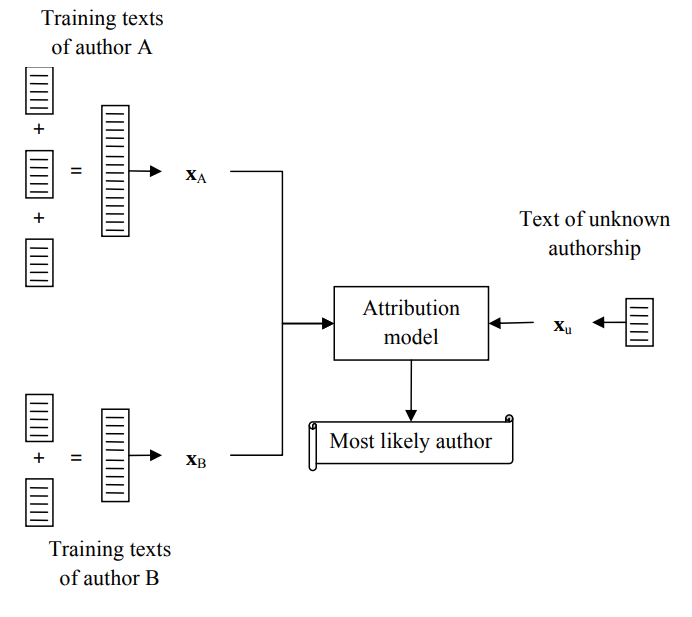
\includegraphics[scale=0.4]{./pictures/method/profile_based.png}
    \caption{Illustrate the typical profile based Authorship Verification or
        Authorship Attribution setup.\cite{stamatos2009} The texts of each
        author are combined using some combination function such as an average
        or a concatenation. Those \textit{profiles} are then given to a Machine
        Learning model to train. The output is a model which is used to predict
        unknown texts. }

    \label{fig:profile_based}
\end{figure}

We will generally use the instance based approach. The reason we use an instance
based approach is that it allows us to use extra information from each single
text. For example writing style may change over time especially for secondary
school pupils that evolve very much in a short amount of time. Since we use an
instance based approach we are able to weight similarity to newer texts higher
than similarity to older texts.

There are also another split between methods that we consider. There are
generalizing and author specific models. In a generalizing model only a single
model is trained on data from multiple authors and are able to make predictions
about previously unseen authors. In the author specific model a separate model
has to be trained for each author and is not able to make predictions for
previously unseen authors. The generalizing model has several advantages, it
only has to be trained once and after that it can be used for everyone and
it can make use of big data since it can use data from several authors for
training. The author specific model has the advantage that it can better fit
to the specific quirks of a particular author since it is trained separately
for each author. The downside of the author specific approach is that a new
model has to be trained for each new author. We will focus on the generalizing
approach since it is easier to implement for MaCom as they only have to train a
model once.

As a unit of measuring the quality of our models, and how well they adhere to
95\% specificity constraint, we will also compute the number of \gls{TP}s,
\gls{TN}s, \gls{FP}s and \gls{FN}s, as was done in a project previously created
by us.\cite{US} In these problems we get,

\begin{itemize}
    \item a \gls{TP} whenever we answer \textit{True} and the texts are written
        by the same author,
    \item a \gls{TN} whenever we answer \textit{False} and the texts are
        \textbf{not} written by the same author,
    \item a \gls{FP} whenever we answer \textit{True} and the texts are
        \textbf{not} written by the same author,
    \item a \gls{FN} whenever we answer \textit{False} and the texts are written
        by the same author.
\end{itemize}

Given those definitions the \gls{TPR}, \gls{FPR}, \gls{TNR} and \gls{FNR}
describes.

\begin{description}
    \item[\gls{TPR}: ] The fraction of positives that we reported \textit{True}
        on i.e. the fraction of texts written by the same author that we say are
        written by the same author.
    \item[\gls{FPR}: ] The fraction of negatives that we reported \textit{True}
        on i.e. the fraction of texts written by different authors that we say
        are written by the same author.
    \item[\gls{TNR}: ] The fraction of negatives that we reported \textit{False}
        on i.e. the fraction of texts written by different authors that we say
        are written by different authors.
    \item[\gls{FNR}: ] The fraction of positives that we reported \textit{False}
        on i.e. the fraction of texts written by the same author that we say are
        written by different authors.
\end{description}

And they can be computed as,

\begin{align}
    TPR &= \frac{TP}{TP + FN}, \\
    FPR &= \frac{FP}{FP + TN}, \\
    TNR &= \frac{TN}{TN + FP}, \\
    FNR &= \frac{FN}{FN + TP}.
\end{align}

In the case of MaCom, we want to minimize the \gls{FNR} as much as possible, so
as to not wrongfully accuse anyone of not having written their assignment.


\subsection{Deep Learning}

In this paper we will approach the authorship verification/attribution problem
using deep-learning. The terms of deep learning, it was first introduced to
machine machine learning in 1989, and afterward to \gls{NN}'s in 2000. The terms
quickly became synonymous with \gls{NN}'s due to them being some of the more
efficient deep learning methods.\cite{Schmidhuber:2015}

With the inner workings of the brain used as the basis, a standard simple
\gls{NN} consists of a set interconnected processors, called neurons. Each of
these neurons has a real-valued activation associated with it, which activates
differently depending on the specific neuron. The input neurons activate through
perceiving the environment, or in other words, when it is fed data externally.
Other neurons are simply activated through the weighted activation of previous
neurons. More details regarding these weights will be presented later in the
paper.\cite{DBLP:journals/corr/Schmidhuber14}

\gls{NN}'s have been around since the 1940's. However, back then they were
merely variations of the linear regressors used at the time, and wasn't
very reminiscent of the Networks on can see today. It wasn't until the
late 1960's, early 70's, that networks comparable to the more modern
approaches surfaced. Examples of such early works, are the two publications
\cite{ivakhnenko1973cybernetic} and \cite{4308320}, which describe multi-layered
feed-forward supervised neural network architectures. While the work described
in \cite{4308320} was indeed one of the first cases of the modern \gls{NN},
actually getting the network to learn was still a problem, as the tweaking of
individual weights attributed to each neuron in the network wasn't trivial.
Little did they know, research to solve that problem was already in progress.
The basics of continuous \gls{BP} was initially described in 1960, in
\cite{Kelley1960}, quickly followed by a simpler approach which used only the
chain rule in 1962, \cite{DREYFUS196230}. It wasn't until 1970 that the modern
version of \gls{BP} was described, using automatic differentiation as its
basis. With this, the increase in research of usages of \gls{BP} increased the
following decades. As the computational power increased several 1000 folds in
the 90's and 2000's, so did the practical usage of \gls{BP}, and \gls{NN} in
general\cite{Schmidhuber:2015}. The real life application of \gls{BP}, will be described
in section \ref{sec:BP}

Like with the history of authorship attribution, research in this area of
science picked up more interest, as we entered the modern computational age,
and with the introduction of the \gls{CNN}. \gls{CNN}s bases themselves on
the early work described in \cite{TJP:TJP19681951215}. They showed that cats
and monkeys visual cortexes contain a set of neurons, each individually
responding to a receptive field, or area, of their field of view. Neighboring
receptive fields all have a certain amount of overlap, however in the end
a cohesive view is created. This is what paved the way for neocognition in
1980\cite{Fukushima1980}, the basis of \gls{CNN}'s, which works in a very
similar manner, looking at overlapping subsections of data. These convolutional
neurons however were rarely used alone, but together with a down-sampling neuron
such as Max Pooling introduced in 1993.\cite{Schmidhuber:2015}

\subsubsection{Neurons}

As mentioned previously a \gls{NN} consists of a collection of neurons. Each
neuron is a simplified mathematical model, which behaves much like neurons in
the brain would, receiving, processing and transmitting data/information. Each
neuron has a set of inputs called $x_i$ and a single output called $z_i$. The
neurons compute a weighted sum of its inputs and applies an activation function
$h$ to the weighted sum. The weights are called $w_i$. The function each neuron
computes is then,

\begin{equation}
    z_i = h\left(
        \sum_{i = 1}^d w_ix_i + w_0
    \right).
\end{equation}

The training of a \gls{NN} consists of changing the weights applied at each
neuron, with the goal of modeling the relationships present in the data.

\subsubsection{Backpropagation}\label{sec:BP}
The actual modeling and learning that the \gls{NN} does, can be attributed
to \gls{BP}. It by this process, that the weight in our \gls{NN} are updated,
signifying the learning the network does. The process can be split into three
steps, which are continuously repeated:
\begin{enumerate}
    \item Feed Forward
    \item Back Propagate
    \item Update Weights
\end{enumerate}
When starting out, we have a set of our starting weight. As to how these weights
are initialized is up to the user. At this point steps 


TODO: More details needed here


\subsubsection{Activation Functions}
The activation function $h$, used at each neuron, defines the output of the
node given a certain input. A simple example of this would be computer chip
circuit, which can be seen as a series of activation functions outputting 0 or
1 depending on their input. This activation function would be a linear one.
When applying activation functions to neurons in \gls{NN}s, they are usually
non-linear, as it allows for the computation of more complex problems using a
smaller amount of neurons, relative to usage of a linear activation function,
as they allow for the universal function approximation, a point also made by
\cite{6797088}

A plot of different activation functions is shown in Figure
\ref{fig:activation_functions}.

\begin{figure}
    \centering
    \textbf{Activation Functions}\par\medskip
    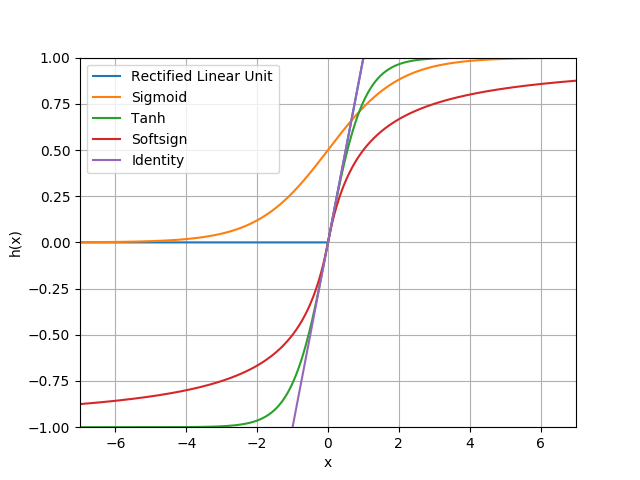
\includegraphics[width=0.5\textwidth]{./pictures/method/activation_functions.png}
    \caption{Different activation functions that can be used in neural
        networks.}
    \label{fig:activation_functions}
\end{figure}

Each activation function has its pros and cons. We mainly made use of the
\gls{ReLu} activation function in the hidden layers of our networks. The
reason for this selection is its general purpose use. When selecting an
activation function for your neurons, the best function would be the one which
best approximates the underlying function. Without a good idea as to what
that function might be, \gls{ReLu} is a good starting point. Its simplicity
provides a quick computation time, and its below zero limitation means that a
large portion of the network won't be activating, resulting in an even smaller
computation time. In addition to that, the derivative of the function is 1
in the case of a positive input, resulting in the \gls{BP} loss having equal
influence throughout the network. In the case of other activation functions,
this might not be the case, resulting in an altering of the error as we
propagate backwards through the network. This could lead to a big error in the
deeper layers not reaching the shallow layers of the network. This property of
the \gls{ReLu} activation function, does however not come without its costs.
If the learning rate of the network isn't configured correctly, a \gls{ReLu}
activated neuron might be blasted with a gradient so large, that it never
reaches a point of activation again. In other words, the neuron "dies". As
such, one can risk a network containing a lot of dead non-activation neurons,
thus greatly decreasing its quality. On the other hand the sigmoid function,
doesn't allow its neurons to die. It can become victim to saturation. In
the case of weight being too small or too high, the output values will be
placed at the far ends of the sigmoid range of values. At this point the
gradient is incredibly small, meaning that the contribution that neuron now has
is negligible. This neuron is now only a strain on the network, slowing it
down through its activation, but contribution nothing, a problem \gls{ReLu}
does not have. Its based on these considerations we chose the \gls{ReLu}
activation function, leaving us the task of properly selecting our learning
rate.\cite{JiYan}\cite{AndrejKarpathy}\cite{AvinashSharmaV}

As the activation function of our output neurons we have generally
used the softmax function. The softmax function is shown in Figure
\ref{fig:softmax_activation}. The function is defined as

\begin{equation}
    h(x_i) = \frac{e^{x_i}}{\sum_{k=1}^n e^{x_k}}, \text{for $i = 1 \dots n$}.
\end{equation}

The softmax function takes any vector $x \in \mathbb{R}^n$ and returns a vector
$y \in (0, 1)^n$. Where the sum of the output vectors elements will be equal to
1. The function is therefore great at constructing a probability distribution
based on an input vector. Each individual value in the vector get a high
probability if the value is high and a low probability if the value is low.
Therefore the function is often used at the end of networks to get the
probability of each class in a classification problem.

\begin{figure}
    \centering
    \textbf{Softmax Activation Function}\par\medskip
    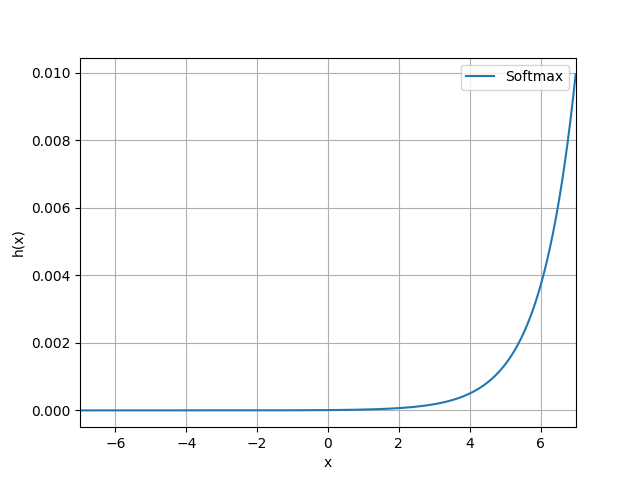
\includegraphics[width=0.5\textwidth]{./pictures/method/softmax_function.png}
    \caption{The softmax activation function.}
    \label{fig:softmax_activation}
\end{figure}





\subsection{Baseline Methods}

In order to gauge the efficiency of our deep learning approaches, we have
chosen to implement some baseline methods. These methods were picked
based on their performance in a previous project written by us as well,
\cite{US}. Albeit that project was only concerned with English texts
provided by the \cite{pan:2015}, and \cite{pan:2014} text forensics tasks,
we hypothesize that the performance of these approaches will perform just
as well on Danish texts when being tuned for the Danish language.


\subsubsection{Extended Delta Method}

One of the best performing methods of \cite{US} was the extended delta method.
As the name suggests the method extends the already existing delta method
described by \cite{evert2015towards}. The normal delta methods consists of first
extracting word frequencies from all texts and using these as the describing
features. After doing this to the entire sample space of texts, and applying a
linear transformation to their respective feature-sets, \gls{KNN} is then used
to determine the author of the introduced texts based on its closest neighbors
in the word-frequency feature-space. The extended delta method, simply expands
on the set of possible features to pick from, rather than being limited to only
using the word-frequencies of the text.


\subsubsection{Author Specific SVM}

Another algorithm used in \cite{US}. Heavily inspired by \cite{hansen2014}
starts out by fetching all texts known to be written by a specific author and an
equal number of texts known not to be written by that same author. It is upon
the feature-set extracted from these texts that a \gls{SVM} is trained, allowing
it to learn the specific author's writing style from the known texts supplied
and in contrast what the writing style of someone not him is. When a new text,
with disputed authorship is presented the hope is that the trained \gls{SVM}
will be able to determine if the author it was trained on, is in fact the author
of this new text as well.


\subsection{Siamese Neural Network - Iteration 1}

% TODO: Maybe make clearer what exactly were our idea and what we have from the
% three articles.

Our idea for our first network architecture was to use a similar architecture
as the ones used in \cite{Koch2015SiameseNN}, \cite{NIPS1993_769} and
\cite{qian:2018}. In our implementation we use a combination of the three
approaches. Our main idea was to combine the approaches of \cite{qian:2018}
and \cite{Koch2015SiameseNN}. \cite{qian:2018} use a Siamese network but
with no convolutions and a distance function on top for text analysis while
\cite{Koch2015SiameseNN} used a Siamese network with convolutions and fully
connected network on top for image analysis. Our approach is to use convolutions
in the Siamese network to learn important features from the texts. We also use
a fully connected network on top of the convolutional layers to learn from the
features the convolution extracted. In more detail we start by preprocessing
our input data. The input consists of a set of utf-8 encoded texts with an
associated author id. To limit the number of different characters our network
has to deal with we map all characters that occur with a frequency of less than
$\frac{1}{100,000}$ to a garbage character we define. Since our network can only
handle inputs of the same length we pad all texts to have the length of the
longest text with another garbage character. We map all other characters to the
numbers 1 to the size of the character set.

Now we have a set of vectors of numbers of the same size each associated with
an author id. To construct an authorship verification dataset we looped through
all the vectors. For each vector we drew a random vector of the same author and
a random vector of a different author. We then created two problem instances we
could train on. One instance of two vectors from the same author with a label of
1 and one instance of two vectors from different authors with a label of 0. We
split the list of problems into two sets. A validation set consisting of 20\% of
the problems and a training set consisting of 80\% of the problems.

The network we used to try and solve the problem is shown in Figure
\ref{fig:network_1}. The Siamese part of the network is the Convolutional
Layer. We used 1000 filters of size 10. That means that 1000 different features
are supposed to be learned by the network and each feature can use a local
context of 10 characters to extract a feature. After the convolution we have a
max-over-time pooling layer. The layer takes the maximum value of each feature
such that we have 1000 features from each text. We then have a normal dense
neural network on top of that which are given the features of both texts. The
dense network is then supposed to learn how to compare the features from the two
texts. We have 1 dense hidden layer each with 500 neurons. At the end we have
a output layer with two outputs. The activation function for all layers except
the last one is the rectified linear unit and the activation function of the
last layer is the softmax function. The output of the network is a probability
distribution over the two classes.

The input to the network first goes through an embedding layer. The embedding
layer transforms integers into dense vectors of floating point numbers. The
embedding layer functions as a lookup table such that each integer is mapped
to the same dense vector. The embedding is trainable meaning that better
embeddings will be learned while the network is training. The different layers
perform the following tasks,

\begin{description}
    \item[known\_input:] The input of the known text. The known text consist of
        an array of numbers where each number corresponds to a unique character.
        Characters that occur less frequently than $\frac{1}{100000}$ are
        replaced by a special number. The texts are padded to the same length
        with another special number.
    \item[unknown\_input:] The input of the unknown text. The unknown text
        consist of an array of numbers where each number corresponds to a unique
        character. Characters that occur less frequently than $\frac{1}{100000}$
        are replaced by a special number. The texts are padded to the same
        length with another special number.
    \item[embedding\_1:] The layer takes an array of numbers and encodes them as
        dense vectors of some size. Our embedding layer encodes each number as a
        5 dimensional vector. The embedding is learnable meaning that characters
        that are alike will be mapped to roughly similar positions in the output
        space. For example we expect the characters 'a' and 'A' to mapped closer
        to each other than 'a' and 'b'.
    \item[convolustion\_10:] A convolutional layer with 1000 filters and a
        kernel size of 10. The convolutional window will slide over the embedded
        characters looking at 10 at a time. For each 10 characters we will get a
        single output. The stride is 1 so the output of the layer will only be
        10 units shorter than the input.
    \item[repr\_known:] The representation of the known text is the
        max-over-time pooling of the convolutional layers output. Since 1000
        filters were used in the convolutional layer the representation of the
        known text will consist of 1000 numbers.
    \item[repr\_unknown:] The representation of the unknown text is the
        max-over-time pooling of the convolutional layers output. Since 1000
        filters were used in the convolutional layer the representation of the
        unknown text will consist of 1000 numbers.
    \item[concatenate\_1:] Merge the two representations together by doing a
        concatenation of the $2 \times 1000$ features extracted giving a single
        vector of $2000$ values.
    \item[dense\_1:] Fully connected layer with 500 neurons. All 500 neurons is
        connected to the 2000 values from the concatenation layer. The
        activation function is the \gls{ReLu}.
    \item[output:] The output layer consisting of two neurons. Each of them is
        connected to the 500 neurons in dense\_1. The activation function is the
        softmax function. The first neuron computes the probability of the two
        texts being written by different people. The second neuron computes the
        probability of the two texts being written by the same person.
\end{description}

\begin{figure}[htb]
    \centering
    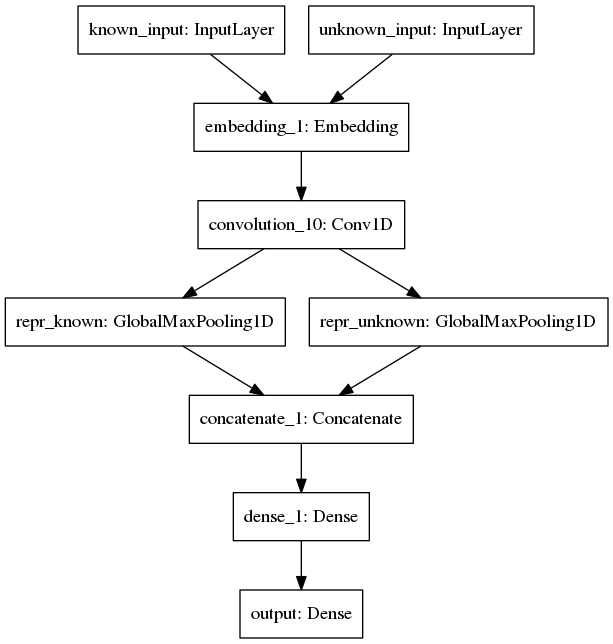
\includegraphics[width=0.6\textwidth]{./pictures/method/network1.png}
    \caption{Illustrate the structure of our first Siamese Neural Network
        Architecture.}
    \label{fig:network_1}
\end{figure}

The network obtained a validation accuracy of 0.68684. We have shown both the
training and validation accuracies in the different epochs in Figure
\ref{fig:network1_accuracies}. In that plot we can see that the network very
quickly overfits the training data and no longer learns anything general.

\begin{figure}[htb]
    \centering
    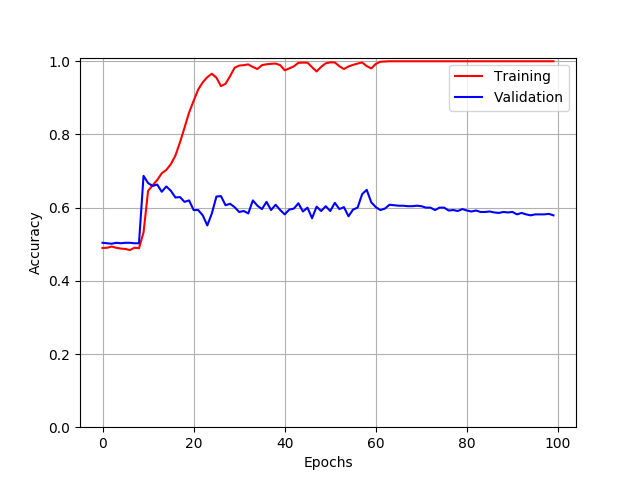
\includegraphics[width=0.5\textwidth]{./pictures/method/network_1_accuracies.png}
    \caption{Training and validation accuracies for the iteration 1 network in
        the different epochs of the networks execution.}
    \label{fig:network1_accuracies}
\end{figure}

Validation true positives 269

Validation true negatives 253

Validation false positives 109

Validation false negatives 129


\subsection{Siamese Neural Network - Iteration 2}

% TODO: Illustrate how dropout corresponds to training different subnetworks in
% each iteration.

In our last network we observed that the network after a few number of epochs
overfitted on the training dataset. The validation accuracy quickly began
stalling as the training accuracy went to 100\%. We therefore focused our
second network architecture on limiting overfitting. We added a dropout layer
before the output layer. The layer prevents overfitting by making sure that
the network cannot rely on the output of all neurons during training. This
unpredictability makes it harder for the network to learn specific quirks of
the training dataset since small quirks will only be picked up by a small
amount of neurons while larger trends will be represented by a larger set
of neurons. \cite{JMLR:v15:srivastava14a} investigated the use of dropout
layers in different problem settings. They found that dropout layers reduced
overfitting in all problems they looked at. In particular they found that
document classification which is similar to what we are doing were also
improved. The main drawback of a dropout layer is that it increase the run time
of training the networks (\cite{JMLR:v15:srivastava14a}).

In iteration 1 the function we used to merge features from the known and unknown
text together were a concatenation. If we let the extracted features of the
known text be $K_i$ and the extracted features of the unknown text be $U_i$ then
$K_0$ and $U_0$ correspond to the same feature extracted from the two texts. The
concatenation merge function would then produce,

\begin{equation}
    merge(K, U) \rightarrow \left(
        K_0, K_1, \dots, K_n, U_0, U_1, \dots, U_n
    \right)^T.
\end{equation}

That means that the neural network would have to figure out by itself that input
$0$ were related in particular to input $n + 1$. To save the network that task
we also replaced the merging function to the absolute difference of the feature
vectors. That means that our merge function became,

\begin{equation}
    merge(K, U) \rightarrow \left(
        (|K_0 - U_0|), (|K_1 - U_1|), \dots, (|K_n - U_n|)
    \right)^T.
\end{equation}

So the network no longer has to learn arbitrary indexes. Instead it can learn
which features is important for authorship verification and learn thresholds for
when each feature is important. With the new merging we will have a large number
whenever the two features are far apart and a small number whenever they are
close to each other.

We changed the convolutional filters we used from 1000 convolutional filters of
size 10 to 500 convolutional filters of size 4 and 500 convolutional filters of
size 8. The idea was that the filters could learn different features where some
of the features would consist of a large number of characters and other of the
features would consist of a small number of characters. The architecture of our
network from iteration 2 is shown in Figure \ref{fig:network_2}. The layers are,

\begin{description}
    \item[known\_input:] The input of the known text. The known text consist of
        an array of numbers where each number corresponds to a unique character.
        Characters that occur less frequently than $\frac{1}{100000}$ are
        replaced by a special number. The texts are padded to the same length
        with another special number.
    \item[unknown\_input:] The input of the unknown text. The unknown text
        consist of an array of numbers where each number corresponds to a unique
        character. Characters that occur less frequently than $\frac{1}{100000}$
        are replaced by a special number. The texts are padded to the same
        length with another special number.
    \item[embedding\_1:] The layer takes an array of numbers and encodes them as
        dense vectors of some size. Our embedding layer encodes each number as a
        5 dimensional vector. The embedding is learnable meaning that characters
        that are alike will be mapped to roughly similar positions in the output
        space. For example we expect the characters 'a' and 'A' to mapped closer
        to each other than 'a' and 'b'.
    \item[convolustion\_8:] A convolutional layer with 500 filters and a
        kernel size of 8. The convolutional window will slide over the embedded
        characters looking at 8 at a time. For each 8 characters we will get a
        single output. The stride is 1 so the output of the layer will only be
        8 units shorter than the input.
    \item[convolustion\_4:] A convolutional layer with 500 filters and a
        kernel size of 4. The convolutional window will slide over the embedded
        characters looking at 4 at a time. For each 4 characters we will get a
        single output. The stride is 1 so the output of the layer will only be
        4 units shorter than the input.
    \item[known\_repr\_8:] The representation of the known text is the
        max-over-time pooling of the convolutional\_8 layers output. Since 500
        filters were used in the convolutional\_8 layer the representation of
        the known text will consist of 500 numbers.
    \item[unknown\_repr\_8:] The representation of the unknown text is the
        max-over-time pooling of the convolutional\_8 layers output. Since 500
        filters were used in the convolutional\_8 layer the representation of
        the unknown text will consist of 500 numbers.
    \item[known\_repr\_4:] The representation of the known text is the
        max-over-time pooling of the convolutional\_4 layers output. Since 500
        filters were used in the convolutional\_4 layer the representation of
        the known text will consist of 500 numbers.
    \item[unknown\_repr\_4:] The representation of the unknown text is the
        max-over-time pooling of the convolutional\_4 layers output. Since 500
        filters were used in the convolutional\_4 layer the representation of
        the unknown text will consist of 500 numbers.
    \item[concatenate\_1:] Merge the representation of the features of the known
        text from the convolutional\_8 and convolutional\_4 layers with a
        concatenation function to produce a single feature vector.
    \item[concatenate\_2:] Merge the representation of the features of the
        unknown text from the convolutional\_8 and convolutional\_4 layers with
        a concatenation function to produce a single feature vector.
    \item[absolute\_difference:] Merge the representation of the known and
        unkonwn text with the absolute difference between the vectors. The input
        is the two vectors representing the texts of 1000 elements. The output
        is the elementwise absolute difference.
    \item[dense\_1:] A fully connected layer with 500 neurons. The 500 neurons
        are all connected to all outputs of the absolute\_difference layer. The
        activation function is the \gls{ReLu}.
    \item[dense\_2:] A fully connected layer with 500 neurons. The 500 neurons
        are all connected to all outputs of the previous layer. The
        activation function is the \gls{ReLu}.
    \item[dropout\_1:] A dropout layer with 30\% dropout. In each batch during
        training 30\% of the network is turned of and only the other 70\% is
        trained.
    \item[output:] The output layer consisting of two neurons. Each of them is
        connected to the 500 neurons in dense\_2. The activation function is the
        softmax function. The first neuron computes the probability of the two
        texts being written by different people. The second neuron computes the
        probability of the two texts being written by the same person.
\end{description}

\begin{figure}
    \centering
    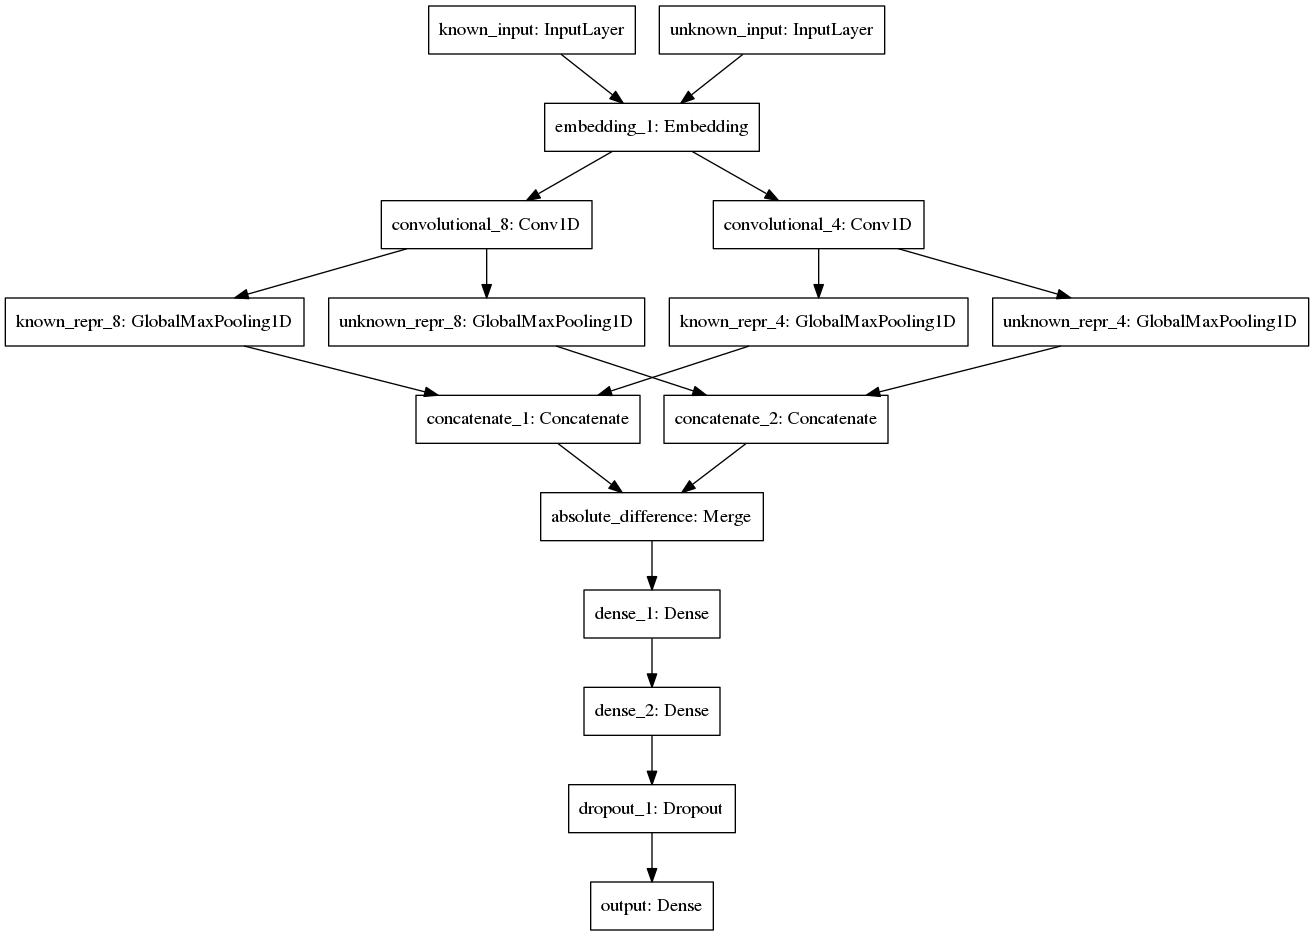
\includegraphics[width=\textwidth]{./pictures/method/network2.png}
    \caption{Illustrate the structure of our second Siamese Neural Network
        Architecture.}
    \label{fig:network_2}
\end{figure}

We also added more dense layers to the model. A plot of the
training and validation accuracies per epoch can be seen in Figure
\ref{fig:network2_accuracies}.

\begin{figure}
    \centering
    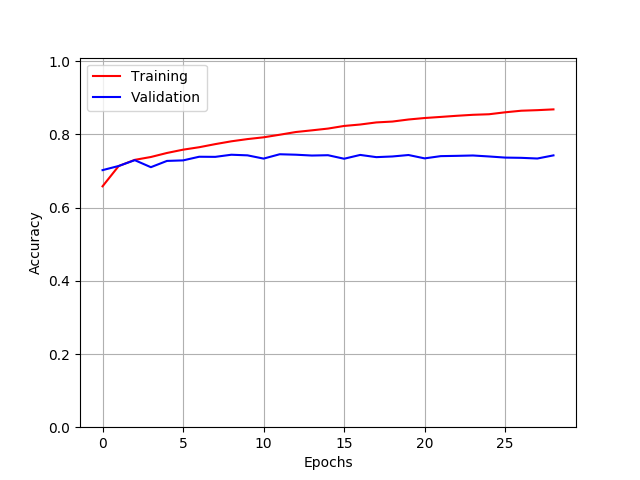
\includegraphics[width=0.5\textwidth]{./pictures/method/network_2_accuracies.png}
    \caption{Shows the training and validation accuracies on the second
        network.}
    \label{fig:network2_accuracies}
\end{figure}

The maximum validation accuracy obtained were 0.74464 in epoch 12.


\subsection{Siamese Neural Network - Iteration 3}

In iteration 2 we observed that the network seemed to learn everything in the
first epoch and didn't improve much after that. We also observed that the
accuracy improved compared to the first network. We therefore wanted to try a
larger network which would be able to hopefully learn more and obtain a higher
accuracy than our first two networks.

We both tried adding more convolutions and adding more dense layers. Our third
network use 700 convolutions of size 8 (currently drawn confusingly) and 500
convolutions of size 4. The network then contains 4 dense layers all with 500
hidden neurons with \gls{ReLu} activation function. Then a dropout layer with
30\% dropout and finally the output layer with 2 neurons and a softmax
activation function. The function we use to combine the features from the two
texts are still the absolute difference as that seemed to work fine for the
previous network. We have shown the structure of the third network in Figure
\ref{fig:network3}. A description of the layers are,

\begin{description}
    \item[known\_input:] The input of the known text. The known text consist of
        an array of numbers where each number corresponds to a unique character.
        Characters that occur less frequently than $\frac{1}{100000}$ are
        replaced by a special number. The texts are padded to the same length
        with another special number.
    \item[unknown\_input:] The input of the unknown text. The unknown text
        consist of an array of numbers where each number corresponds to a unique
        character. Characters that occur less frequently than $\frac{1}{100000}$
        are replaced by a special number. The texts are padded to the same
        length with another special number.
    \item[embedding\_1:] The layer takes an array of numbers and encodes them as
        dense vectors of some size. Our embedding layer encodes each number as a
        5 dimensional vector. The embedding is learnable meaning that characters
        that are alike will be mapped to roughly similar positions in the output
        space. For example we expect the characters 'a' and 'A' to mapped closer
        to each other than 'a' and 'b'.
    \item[convolustion\_8:] A convolutional layer with 700 filters and a
        kernel size of 8. The convolutional window will slide over the embedded
        characters looking at 8 at a time. For each 8 characters we will get a
        single output. The stride is 1 so the output of the layer will only be
        8 units shorter than the input.
    \item[convolustion\_4:] A convolutional layer with 500 filters and a
        kernel size of 4. The convolutional window will slide over the embedded
        characters looking at 4 at a time. For each 4 characters we will get a
        single output. The stride is 1 so the output of the layer will only be
        4 units shorter than the input.
    \item[known\_repr\_8:] The representation of the known text is the
        max-over-time pooling of the convolutional\_8 layers output. Since 700
        filters were used in the convolutional\_8 layer the representation of
        the known text will consist of 700 numbers.
    \item[unknown\_repr\_8:] The representation of the unknown text is the
        max-over-time pooling of the convolutional\_8 layers output. Since 700
        filters were used in the convolutional\_8 layer the representation of
        the unknown text will consist of 700 numbers.
    \item[known\_repr\_4:] The representation of the known text is the
        max-over-time pooling of the convolutional\_4 layers output. Since 500
        filters were used in the convolutional\_4 layer the representation of
        the known text will consist of 500 numbers.
    \item[unknown\_repr\_4:] The representation of the unknown text is the
        max-over-time pooling of the convolutional\_4 layers output. Since 500
        filters were used in the convolutional\_4 layer the representation of
        the unknown text will consist of 500 numbers.
    \item[concatenate\_1:] Merge the representation of the features of the known
        text from the convolutional\_8 and convolutional\_4 layers with a
        concatenation function to produce a single feature vector.
    \item[concatenate\_2:] Merge the representation of the features of the
        unknown text from the convolutional\_8 and convolutional\_4 layers with
        a concatenation function to produce a single feature vector.
    \item[absolute\_difference:] Merge the representation of the known and
        unkonwn text with the absolute difference between the vectors. The input
        is the two vectors representing the texts of 1200 elements. The output
        is the elementwise absolute difference.
    \item[dense\_1:] A fully connected layer with 500 neurons. The 500 neurons
        are all connected to all outputs of the absolute\_difference layer. The
        activation function is the \gls{ReLu}.
    \item[dense\_2:] A fully connected layer with 500 neurons. The 500 neurons
        are all connected to all outputs of the previous layer. The
        activation function is the \gls{ReLu}.
    \item[dense\_3:] A fully connected layer with 500 neurons. The 500 neurons
        are all connected to all outputs of the previous layer. The
        activation function is the \gls{ReLu}.
    \item[dense\_4:] A fully connected layer with 500 neurons. The 500 neurons
        are all connected to all outputs of the previous layer. The
        activation function is the \gls{ReLu}.
    \item[dropout\_1:] A dropout layer with 30\% dropout. In each batch during
        training 30\% of the network is turned of and only the other 70\% is
        trained.
    \item[output:] The output layer consisting of two neurons. Each of them is
        connected to the 500 neurons in dense\_4. The activation function is the
        softmax function. The first neuron computes the probability of the two
        texts being written by different people. The second neuron computes the
        probability of the two texts being written by the same person.
\end{description}

\begin{figure}
    \centering
    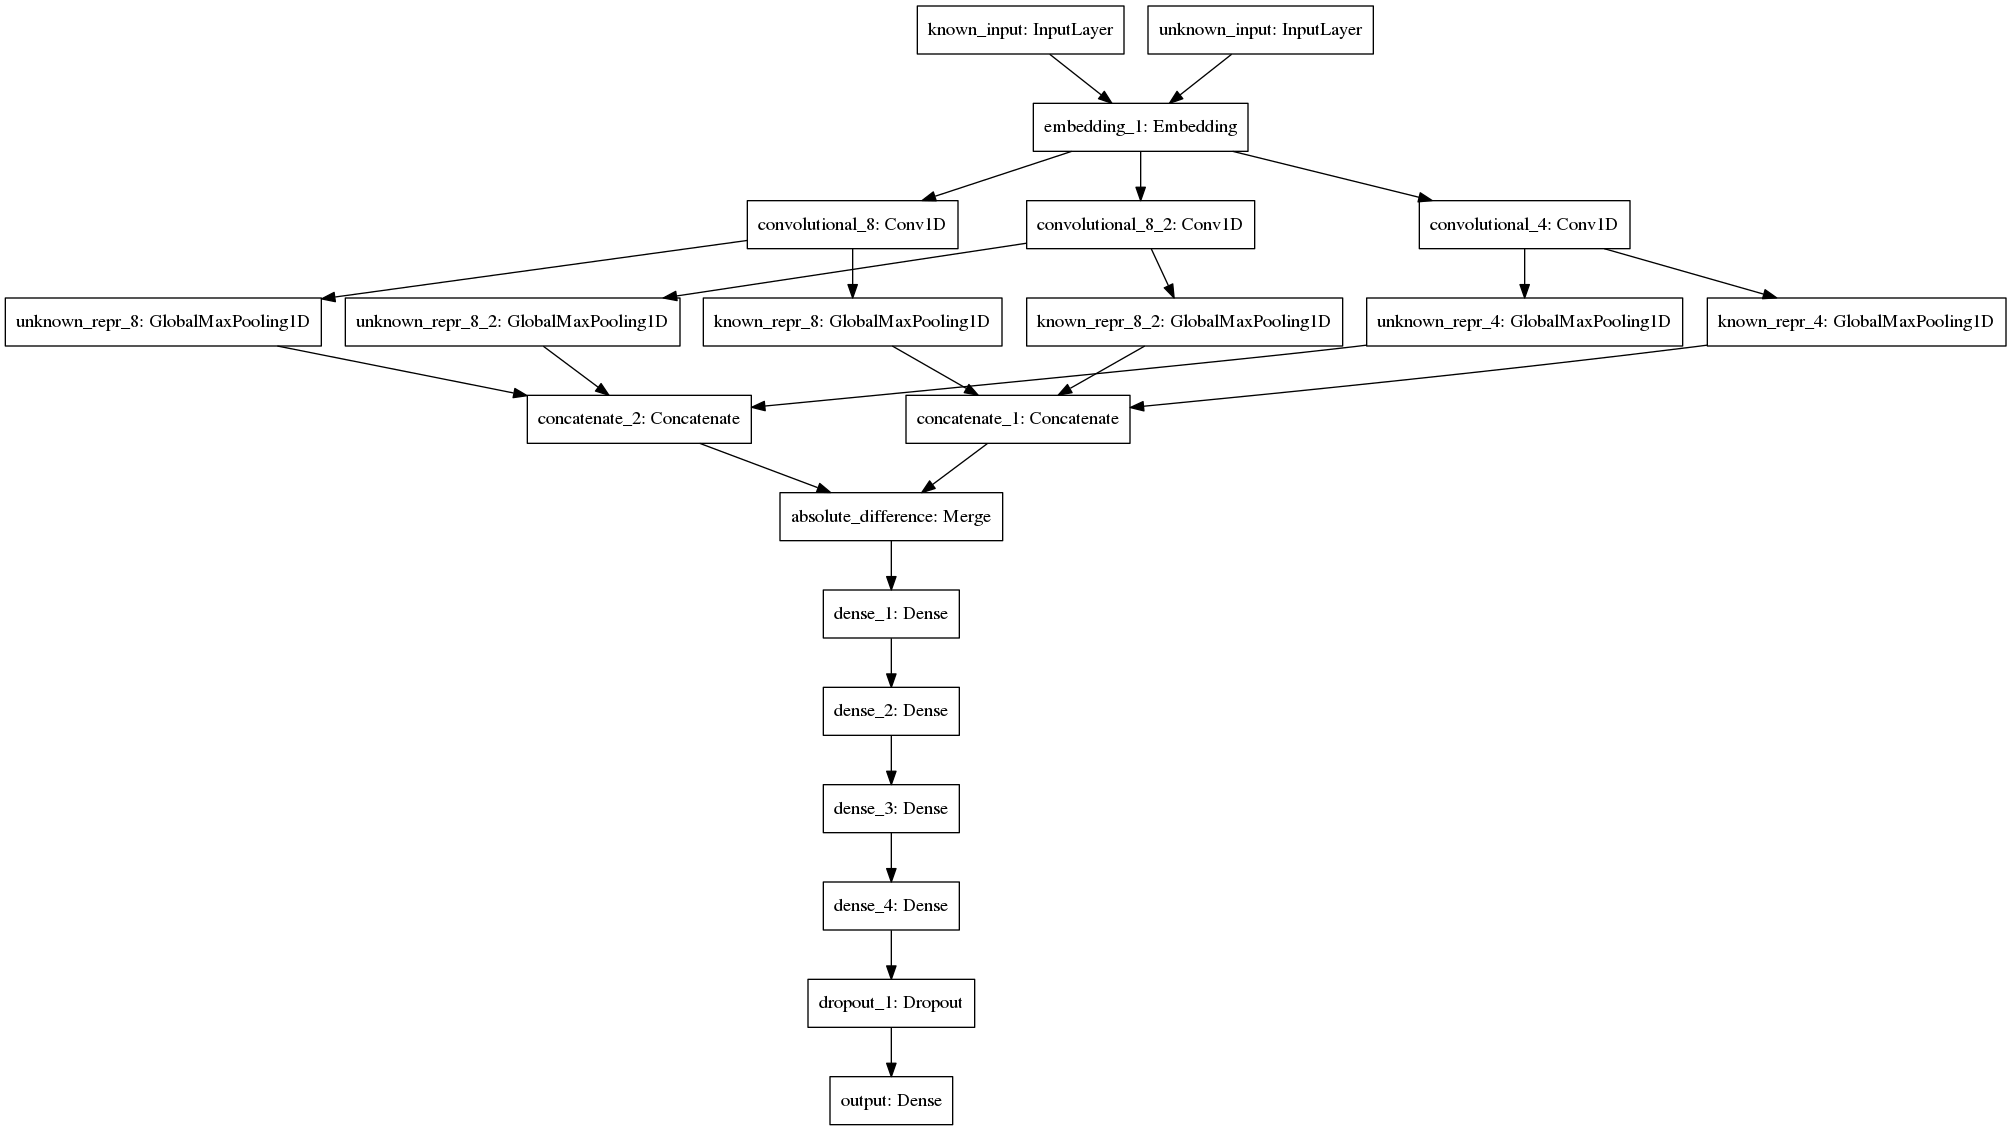
\includegraphics[width=\textwidth]{./pictures/method/network3.png}
    \caption{Illustrate the structure of our third Siamese Neural Network.}
    \label{fig:network3}
\end{figure}

Our third network were able to obtain an accuracy of 0.83612. We have shown the
training and validation accuracies in Figure \ref{fig:network_3_accuracies}. We
can see that the network quickly improve the about 80\% accuracy and after that
not much happens.

\begin{figure}
    \centering
    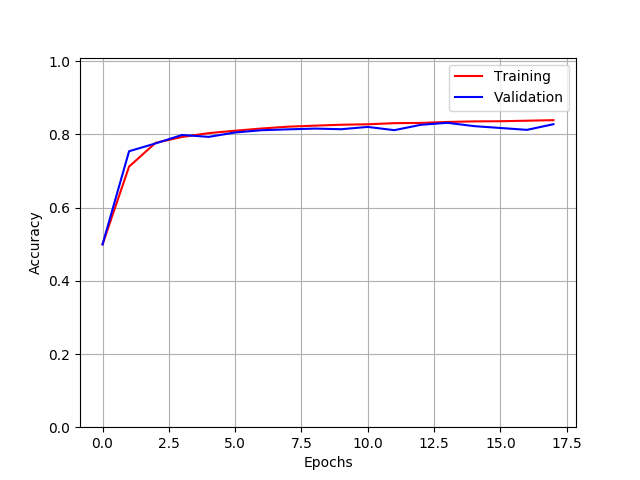
\includegraphics[width=0.5\textwidth]{./pictures/method/network_3_accuracies.png}
    \caption{Shows the training and validation accuracies over the epochs of
        training on the third network.}
    \label{fig:network_3_accuracies}
\end{figure}

To get an idea of which features the network were looking at we looked at the
output of the convolutional layers. After the convolutional layers we have a
max-over-time pool so we know that higher values are important. We could then
take a text, feed it to the network, find the index of the maximum output of
the convolutional layers and then show the text snipped (char-n-gram) that
produced that high value. We then did that for all the texts in the dataset. The
first filter in the network for example yielded many short strings ending with 3
newlines. Some examples of these are,

\begin{lstlisting}[gobble=4]
    'adsen\n\n\n'
    'ndsen\n\n\n'
    'umeer\n\n\n'
    'endte\n\n\n'
    'ingen\n\n\n'
    'ehren\n\n\n'
    'elsen\n\n\n'
    'ommer\n\n\n'
    'Ruter\n\n\n'
    'ummer\n\n\n'
    'ersen\n\n\n'
    'ansen\n\n\n'
    'heden\n\n\n'
    'ensen\n\n\n'
    'arsen\n\n\n'
    'orten\n\n\n'
    'ulsen\n\n\n'
    'orgen\n\n\n'
\end{lstlisting}

Many of those short string looks like the ending of common Danish
names followed by three newlines. Here are some examples of the
names taken from a list of the 100 most frequent surnames in Denmark
\footnote{http://www.mydanishroots.com/surnames-meaning-and-origin/the-100-most-
common-surnames-in-denmark.html},

\begin{description}
    \item[adsen:] Madsen.
    \item[ndsen:] Svendsen, Frandsen.
    \item[elsen:] Nielsen, Mikkelsen.
    \item[ersen:] Pedersen, Andersen, Petersen, Iversen, Jespersen.
    \item[ansen:] Hansen, Christiansen, Johansen, Kristiansen.
    \item[ensen:] Jensen, Christensen, S\o rensen, J\o rgensen, Kristensen,
        Mortensen, Mogensen.
    \item[arsen:] Larsen.
    \item[ulsen:] Poulsen.
\end{description}

The network therefore seems to have learned that a name followed by whitespace
are an important feature when determining the authorship of a text. Clearly when
a student buy an assignment from a ghost writer the text will contain the
students own name. Therefore these features are counter productive since the
network learns that as a result of how we have created the training dataset
where each text has the correct authors name in it.

Things we are considering to do:
\begin{itemize}
    \item Filter out names from texts. Mikkel is currently on vacation and he
        did not make a new extract for us before he left. He agreed to perform
        an extract while he is on vacation. The new extract will either give us
        the name of the student writing the assignment or Mikkel will filter out
        the names from the texts for us.
    \item Cut texts into smaller pieces. Since only the first piece will contain
        the students name the network can no longer rely heavily on learning
        name based features. That will also result in a shorter training time
        since we can run with a larger batch size.
    \item Get better idea of what the networks are reacting to by looking at
        more than just the first filter. Obviously we cannot go through them all
        since there are several thousand.
\end{itemize}


\subsection{Prediction System}

The networks we have trained above does not solve the problem presented to us
by MaCom. The networks above all compare two texts and predict whether or not
they have been written by the same person. In the MaCom problem we are given a
set of texts for each author so we can make use of all texts when making our
predictions. We can also use metadata about the individual texts to make our
prediction. We can for example weigh the newest texts higher authorship than
the older texts. As described earlier writing style changes over time and it is
therefore clear that newer texts captures more of an authors current writing
style than older. An advantage of using multiple texts for each author to make a
prediction is that outliers will be averaged out.

The scheme we have implemented is using the networks we trained previously
to predict all texts of an author and then take a weighted average over the
probabilities of the predictions. More formally given a text $x$, a trained
neural network $N$ and an author $\alpha$ with $n$ previous texts we will verify
whether or not $x$ is written by $\alpha$ by using the network to compare each
$t \in T(\alpha)$ to $x$. That gives us $n$ probabilities $P_i$ of the text
$x$ being written by the same author as each $t \in T(\alpha)$. We then take a
weighted average over $P$ to obtain a final probability $p$. We then threshold
that final probability such that we don't accuse to many people of cheating.

Taking the network $N$ as network 3 and thresholding the final probability as
$0.5$ we obtained an accuracy of 0.92452 with 1934 \gls{TP}'s, 1851 \gls{TN}'s,
196 \gls{FP}'s and 113 \gls{FN}'s. The results come from taking each author
$\alpha$ in our dataset (concatenation of both training and validation),
randomly taking a text $t_k \in T(\alpha)$ and a text
$t_u \in \bigcup_{\beta \in A} T(\beta) \setminus T(\alpha)$ and then applying
the prediction system first to $T(\alpha) \setminus \{t_k\}$ and $t_k$ and then
to $T(\alpha) \setminus \{t_k\}$ and $t_u$. In this experiment the fraction of
wrongfull accusations out of all accusations are $\frac{FNS}{FNS + TNS} =
\frac{113}{113 + 1851} = 0.057535$. That is an excellent result since that means
that less than 10\% of the accusations we make will be wrong.

TODO:
\begin{itemize}
    \item Describe Backpropagration
    \item Describe Optimizers
    \item Describe Convolutions
    \item Describe Dropout
    \item Describe RNN
    \item Use squared distance as merge function to get larger differences
        between close and far apart.
    \item Try to not use dense network but a distance metric.
\end{itemize}
